% !TeX spellcheck = da_DK
%implementing document formatting:
\documentclass[a4paper,11pt,fleqn,dvipsnames,twoside,openany]{memoir} 	% Openright aabner kapitler paa hoejresider (openany begge) openany skal laves om til openright, hvis man ønske blanke sider!

%%%% PACKAGES %%%%
\usepackage{pdfpages}
\usepackage{eurosym}
\usepackage{ulem}


% ¤¤ Oversaettelse og tegnsaetning ¤¤ %
\usepackage[utf8]{inputenc}					% Input-indkodning af tegnsaet (UTF8)
\usepackage[danish]{babel}					% Dokumentets sprog
\usepackage[T1]{fontenc}					% Output-indkodning af tegnsaet (T1)
\usepackage{ragged2e,anyfontsize}			% Justering af elementer
\usepackage{fixltx2e}						% Retter forskellige fejl i LaTeX-kernen
																			
% ¤¤ Figurer og tabeller (floats) ¤¤ %
\usepackage{graphicx} 						% Haandtering af eksterne billeder (JPG, PNG, EPS, PDF)
%\usepackage{eso-pic}						% Tilfoej billedekommandoer paa hver side
%\usepackage{wrapfig}						% Indsaettelse af figurer omsvoebt af tekst. \begin{wrapfigure}{Placering}{Stoerrelse}
\usepackage{multirow}                		% Fletning af raekker og kolonner (\multicolumn og \multirow)
\usepackage{multicol}         	        	% Muliggoer output i spalter
\usepackage{rotating}						% Rotation af tekst med \begin{sideways}...\end{sideways}
\usepackage{colortbl} 						% Farver i tabeller (fx \columncolor og \rowcolor)
\usepackage{xcolor}							% Definer farver med \definecolor. Se mere: http://en.wikibooks.org/wiki/LaTeX/Colors
\usepackage{flafter}						% Soerger for at floats ikke optraeder i teksten foer deres reference
\let\newfloat\relax 						% Justering mellem float-pakken og memoir
\usepackage{float}							% Muliggoer eksakt placering af floats, f.eks. \begin{figure}[H]
\usepackage{booktabs}
\usepackage{longtable}

% ¤¤ Matematik mm. ¤¤
\usepackage{amsmath,amssymb,stmaryrd} 		% Avancerede matematik-udvidelser
\usepackage{mathtools}						% Andre matematik- og tegnudvidelser
\usepackage{textcomp}                 		% Symbol-udvidelser (f.eks. promille-tegn med \textperthousand )
\usepackage{rsphrase}						% Kemi-pakke til RS-saetninger, f.eks. \rsphrase{R1}
\usepackage[version=3]{mhchem} 				% Kemi-pakke til flot og let notation af formler, f.eks. \ce{Fe2O3}
\usepackage{siunitx}						% Flot og konsistent praesentation af tal og enheder med \si{enhed} og \SI{tal}{enhed}
\sisetup{output-decimal-marker = {,}}		% Opsaetning af \SI (DE for komma som decimalseparator) 

% ¤¤ Referencer og kilder ¤¤ %
\usepackage[danish]{varioref}				% Muliggoer bl.a. krydshenvisninger med sidetal (\vref)
\usepackage[numbers]{natbib}				% Udvidelse med naturvidenskabelige citationsmodeller
%\usepackage{xr}							% Referencer til eksternt dokument med \externaldocument{<NAVN>}
%\usepackage{glossaries}					% Terminologi- eller symbolliste (se mere i Daleifs Latex-bog)
\usepackage{lastpage}					    % Gør det mulig at refere til sidste side 

% ¤¤ Misc. ¤¤ %
\usepackage{listings}						% Placer kildekode i dokumentet med \begin{lstlisting}...\end{lstlisting}
\usepackage{lipsum}							% Dummy text \lipsum[..]
\usepackage[shortlabels]{enumitem}			% Muliggoer enkelt konfiguration af lister
\usepackage{pdfpages}						% Goer det muligt at inkludere pdf-dokumenter med kommandoen \includepdf[pages={x-y}]{fil.pdf}	
\pdfoptionpdfminorversion=6					% Muliggoer inkludering af pdf dokumenter, af version 1.6 og hoejere
\pretolerance=2500 							% Justering af afstand mellem ord (hoejt tal, mindre orddeling og mere luft mellem ord)

% Kommentarer og rettelser med \fxnote. Med 'final' i stedet for 'draft' udloeser hver note en error i den faerdige rapport.
\usepackage[footnote,draft,danish,silent,nomargin]{fixme}		


%%%% CUSTOM SETTINGS %%%%

% ¤¤ Marginer ¤¤ %
\setlrmarginsandblock{3.5cm}{2.5cm}{*}		% \setlrmarginsandblock{Indbinding}{Kant}{Ratio}
\setulmarginsandblock{2.5cm}{3.0cm}{*}		% \setulmarginsandblock{Top}{Bund}{Ratio}
\checkandfixthelayout 						% Oversaetter vaerdier til brug for andre pakker

%	¤¤ Afsnitsformatering ¤¤ %
\setlength{\parindent}{0mm}           		% Stoerrelse af indryk
\setlength{\parskip}{3mm}          			% Afstand mellem afsnit ved brug af double Enter
\linespread{1,1}							% Linie afstand

% ¤¤ Litteraturlisten ¤¤ %
\bibpunct[,]{[}{]}{;}{a}{,}{,} 				% Definerer de 6 parametre ved Harvard henvisning (bl.a. parantestype og seperatortegn)
\bibliographystyle{bibtex/harvard}			% Udseende af litteraturlisten.

% ¤¤ Indholdsfortegnelse ¤¤ %
\setsecnumdepth{subsection}		 			% Dybden af nummerede overkrifter (part/chapter/section/subsection)
\maxsecnumdepth{subsection}					% Dokumentklassens graense for nummereringsdybde
\settocdepth{subsection} 					% Dybden af indholdsfortegnelsen

% ¤¤ Lister ¤¤ %
\setlist{
  topsep=0pt,								% Vertikal afstand mellem tekst og listen
  itemsep=-1ex,								% Vertikal afstand mellem items
} 

% ¤¤ Visuelle referencer ¤¤ %
\usepackage[colorlinks]{hyperref}			% Danner klikbare referencer (hyperlinks) i dokumentet.
\hypersetup{colorlinks = true,				% Opsaetning af farvede hyperlinks (interne links, citeringer og URL)
    linkcolor = black,
    citecolor = black,
    urlcolor = black
}

% ¤¤ Opsaetning af figur- og tabeltekst ¤¤ %
\captionnamefont{\small\bfseries\itshape}	% Opsaetning af tekstdelen ('Figur' eller 'Tabel')
\captiontitlefont{\small}					% Opsaetning af nummerering
\captiondelim{. }							% Seperator mellem nummerering og figurtekst
\hangcaption								% Venstrejusterer flere-liniers figurtekst under hinanden
\captionwidth{\linewidth}					% Bredden af figurteksten
\setlength{\belowcaptionskip}{0pt}			% Afstand under figurteksten
		
% ¤¤ Opsaetning af listings ¤¤ %

\definecolor{commentGreen}{RGB}{34,139,24}
\definecolor{stringPurple}{RGB}{208,76,239}

\lstset{language=Matlab,					% Sprog
	basicstyle=\ttfamily\scriptsize,		% Opsaetning af teksten
	keywords={for,if,while,else,elseif,		% Noegleord at fremhaeve
			  end,break,return,case,
			  switch,function},
	keywordstyle=\color{blue},				% Opsaetning af noegleord
	commentstyle=\color{commentGreen},		% Opsaetning af kommentarer
	stringstyle=\color{stringPurple},		% Opsaetning af strenge
	showstringspaces=false,					% Mellemrum i strenge enten vist eller blanke
	numbers=left, numberstyle=\tiny,		% Linjenumre
	extendedchars=true, 					% Tillader specielle karakterer
	columns=flexible,						% Kolonnejustering
	breaklines, breakatwhitespace=true,		% Bryd lange linjer
}

% ¤¤ Navngivning ¤¤ %
\addto\captionsdanish{
	\renewcommand\appendixname{Appendiks}
	\renewcommand\contentsname{Indholdsfortegnelse}	
	\renewcommand\appendixpagename{Appendiks}
	\renewcommand\appendixtocname{Appendiks}
	\renewcommand\cftchaptername{\chaptername~}				% Skriver "Kapitel" foran kapitlerne i indholdsfortegnelsen
	\renewcommand\cftappendixname{\appendixname~}			% Skriver "Appendiks" foran appendiks i indholdsfortegnelsen
}

% ¤¤ Kapiteludssende ¤¤ %
\definecolor{numbercolor}{gray}{0.7}		% Definerer en farve til brug til kapiteludseende
\newif\ifchapternonum

\makechapterstyle{jenor}{					% Definerer kapiteludseende frem til ...
  \renewcommand\beforechapskip{0pt}
  \renewcommand\printchaptername{}
  \renewcommand\printchapternum{}
  \renewcommand\printchapternonum{\chapternonumtrue}
  \renewcommand\chaptitlefont{\fontfamily{pbk}\fontseries{db}\fontshape{n}\fontsize{20}{35}\selectfont\raggedright}
  \renewcommand\chapnumfont{\fontfamily{pbk}\fontseries{m}\fontshape{n}\fontsize{0.35in}{0in}\selectfont\color{black}}
  \renewcommand\printchaptertitle[1]{%
    \noindent
    \ifchapternonum
    \begin{tabularx}{\textwidth}{X}
    {\let\\\newline\chaptitlefont ##1\par} 
    \end{tabularx}
    \par\vskip-2.5mm\hrule
    \else
    \begin{tabularx}{\textwidth}{Xl}
    {\parbox[b]{\linewidth}{\chaptitlefont ##1}} & \raisebox{-5pt}{\chapnumfont \thechapter}
    \end{tabularx}
    \par\vskip2mm\hrule
    \fi
  }
}											% ... her

\chapterstyle{jenor}						% Valg af kapiteludseende - Google 'memoir chapter styles' for alternativer

% ¤¤ Sidehoved ¤¤ %

\makepagestyle{AAU}							% Definerer sidehoved og sidefod udseende frem til ...
\makepsmarks{AAU}{%
	\createmark{chapter}{left}{shownumber}{}{. \ }
	\createmark{section}{right}{shownumber}{}{. \ }
	\createplainmark{toc}{both}{\contentsname}
	\createplainmark{lof}{both}{\listfigurename}
	\createplainmark{lot}{both}{\listtablename}
	\createplainmark{bib}{both}{\bibname}
	\createplainmark{index}{both}{\indexname}
	\createplainmark{glossary}{both}{\glossaryname}
}
\nouppercaseheads											% Ingen Caps oenskes

\makeevenhead{AAU}{Gruppe 403}{}{\leftmark}				% Definerer lige siders sidehoved (\makeevenhead{Navn}{Venstre}{Center}{Hoejre})
\makeoddhead{AAU}{\rightmark}{}{Aalborg Universitet}		% Definerer ulige siders sidehoved (\makeoddhead{Navn}{Venstre}{Center}{Hoejre})
\makeevenfoot{AAU}{\thepage}{}{}							% Definerer lige siders sidefod (\makeevenfoot{Navn}{Venstre}{Center}{Hoejre})
\makeoddfoot{AAU}{}{}{\thepage}								% Definerer ulige siders sidefod (\makeoddfoot{Navn}{Venstre}{Center}{Hoejre})
\makeheadrule{AAU}{\textwidth}{0.5pt}						% Tilfoejer en streg under sidehovedets indhold
\makefootrule{AAU}{\textwidth}{0.5pt}{1mm}					% Tilfoejer en streg under sidefodens indhold

\copypagestyle{AAUchap}{AAU}								% Sidehoved for kapitelsider defineres som standardsider, men med blank sidehoved
\makeoddhead{AAUchap}{}{}{}
\makeevenhead{AAUchap}{}{}{}
\makeheadrule{AAUchap}{\textwidth}{0pt}
\aliaspagestyle{chapter}{AAUchap}							% Den ny style vaelges til at gaelde for chapters
															% ... her
															
\pagestyle{AAU}												% Valg af sidehoved og sidefod


%%%% CUSTOM COMMANDS %%%%

% ¤¤ Billede hack ¤¤ %
\newcommand{\figur}[4]{
		\begin{figure}[H] \centering
			\includegraphics[width=#1\textwidth]{billeder/#2}
			\caption{#3}\label{#4}
		\end{figure} 
}

% ¤¤ Specielle tegn ¤¤ %
\newcommand{\decC}{^{\circ}\text{C}}
\newcommand{\dec}{^{\circ}}
\newcommand{\m}{\cdot}


%%%% ORDDELING %%%%

\hyphenation{}
%\documentclass[a4paper,11pt,fleqn,dvipsnames,oneside,openright,oldfontcommands]{memoir} 	% Openright aabner kapitler paa hoejresider (openany begge)


%%%%%%%%% Indsat random
%makes it possible to refer to the name of a chapter rather than just the number.
\usepackage{nameref}
\usepackage{pdfpages}
\usepackage{marvosym}
\usepackage{setspace}
\usepackage{graphicx} % For at sætte 2 billeder ved siden af hinanden

%package for writing program code in latex
\usepackage{listings}
%%%%%%%%%%%%%%%%%%%%%%

% ¤¤ Oversaettelse og tegnsaetning ¤¤ %
\usepackage[T1]{fontenc}					% Output-indkodning af tegnsaet (T1)
\usepackage[danish]{babel}					% Dokumentets sprog
\usepackage[utf8]{inputenc}					% Input-indkodning af tegnsaet (UTF8)
\usepackage{ragged2e,anyfontsize}			% Justering af elementer
\usepackage{fixltx2e}						% Retter forskellige fejl i LaTeX-kernen							
				
																							
% ¤¤ Figurer og tabeller (floats) ¤¤ %
\usepackage{graphicx} 						% Haandtering af eksterne billeder (JPG, PNG, EPS, PDF)
%\usepackage{eso-pic}						% Tilfoej billedekommandoer paa hver side
%\usepackage{wrapfig}						% Indsaettelse af figurer omsvoebt af tekst. \begin{wrapfigure}{Placering}{Stoerrelse}
\usepackage{multirow}                		% Fletning af raekker og kolonner (\multicolumn og \multirow)
\usepackage{multicol}         	        	% Muliggoer output i spalter
\usepackage{rotating}						% Rotation af tekst med \begin{sideways}...\end{sideways}
\usepackage{colortbl} 						% Farver i tabeller (fx \columncolor og \rowcolor)
\usepackage{xcolor}							% Definer farver med \definecolor. Se mere: http://en.wikibooks.org/wiki/LaTeX/Colors
\usepackage{flafter}						% Soerger for at floats ikke optraeder i teksten foer deres reference
\let\newfloat\relax 						% Justering mellem float-pakken og memoir
\usepackage{float}							% Muliggoer eksakt placering af floats, f.eks. \begin{figure}[H]
\usepackage{array,booktabs,xcolor,longtable} % kan lave \hdashline i tabellertabe
\usepackage{arydshln}
\usepackage{tabu}

	
	
% ¤¤ Matematik mm. ¤¤
\usepackage{amsmath , amsthm , amsfonts , amssymb, float, stmaryrd} 		% Avancerede matematik-udvidelser
%\usepackage{mathtools}						% Andre matematik- og tegnudvidelser
\usepackage{textcomp}                 		% Symbol-udvidelser (f.eks. promille-tegn med \textperthousand )
\usepackage{rsphrase}						% Kemi-pakke til RS-saetninger, f.eks. \rsphrase{R1}
\usepackage[version=3]{mhchem} 				% Kemi-pakke til flot og let notation af formler, f.eks. \ce{Fe2O3}
\usepackage{siunitx}						% Flot og konsistent praesentation af tal og enheder med \si{enhed} og \SI{tal}{enhed}
\sisetup{output-decimal-marker = {,}}		% Opsaetning af \SI (DE for komma som decimalseparator) 

% ¤¤ Referencer og kilder ¤¤ %
\usepackage[danish]{varioref}				% Muliggoer bl.a. krydshenvisninger med sidetal (\vref)
\usepackage[numbers]{natbib}				% Udvidelse med naturvidenskabelige citationsmodeller
%\usepackage{xr}							% Referencer til eksternt dokument med \externaldocument{<NAVN>}
%\usepackage{glossaries}					% Terminologi- eller symbolliste (se mere i Daleifs Latex-bog)
\usepackage{lastpage}					% Gør det mulig at refere til sidste side 

% ¤¤ Misc. ¤¤ %
\usepackage{listings}						% Placer kildekode i dokumentet med \begin{lstlisting}...\end{lstlisting}
\usepackage{lipsum}							% Dummy text \lipsum[..]
\usepackage[shortlabels]{enumitem}			% Muliggoer enkelt konfiguration af lister
\usepackage{pdfpages}						% Goer det muligt at inkludere pdf-dokumenter med kommandoen \includepdf[pages={x-y}]{fil.pdf}	
\pdfoptionpdfminorversion=6					% Muliggoer inkludering af pdf dokumenter, af version 1.6 og hoejere
\pretolerance=2500 							% Justering af afstand mellem ord (hoejt tal, mindre orddeling og mere luft mellem ord)


% Kommentarer og rettelser med \fxnote. Med 'final' i stedet for 'draft' udloeser hver note en error i den faerdige rapport.
\usepackage[footnote,draft,danish,silent,nomargin]{fixme}		


%%%% CUSTOM SETTINGS %%%%

% ¤¤ Marginer ¤¤ %
\setlrmarginsandblock{3.0cm}{2.5cm}{*}		% \setlrmarginsandblock{Indbinding}{Kant}{Ratio}
\setulmarginsandblock{2.5cm}{3.0cm}{*}		% \setulmarginsandblock{Top}{Bund}{Ratio}
\checkandfixthelayout 						% Oversaetter vaerdier til brug for andre pakker

%	¤¤ Afsnitsformatering ¤¤ %
\setlength{\parindent}{6mm}           		% Stoerrelse af indryk
\setlength{\parskip}{0mm}          			% Afstand mellem afsnit ved brug af double Enter
\linespread{1,1}							% Linie afstand



% ¤¤ Indholdsfortegnelse ¤¤ %
\setsecnumdepth{subsection}		 			% Dybden af nummerede overkrifter (part/chapter/section/subsection)
\maxsecnumdepth{subsection}					% Dokumentklassens graense for nummereringsdybde
\settocdepth{section} 					% Dybden af indholdsfortegnelsen

% ¤¤ Lister ¤¤ %
\setlist{
  topsep=0pt,								% Vertikal afstand mellem tekst og listen
  itemsep=-1ex,								% Vertikal afstand mellem items
} 

%hyperlinks in the tabel of contents - comment this out before the report is printed.
\usepackage{hyperref}
\hypersetup{
	bookmarks = true,  % Show 'bookmark'-frame in pdf.
	colorlinks = true, % True = colored links, False = framed links.
	citecolor = black,  % Link color for references.
	linkcolor = black,  % Link color in table of contents.
	urlcolor = black,   % Link color for extern URLs.
}

% ¤¤ Opsaetning af figur- og tabeltekst ¤¤ %
\usepackage{caption}
\usepackage{subcaption}
\captionnamefont{\small\bfseries\itshape}	% Opsaetning af tekstdelen ('Figur' eller 'Tabel')
\captiontitlefont{\small}					% Opsaetning af nummerering
\captiondelim{. }							% Seperator mellem nummerering og figurtekst
\hangcaption								% Venstrejusterer flere-liniers figurtekst under hinanden
%\captionwidth{0.9\textwidth}					% Bredden af figurteksten
\setlength{\belowcaptionskip}{0pt}			% Afstand under figurteksten
\captionsetup[figure]{labelfont={bf,it},font={it}} % sætter nummer til fed og kursis. Resten til fed + skriften er mindre end resten
\captionsetup[table]{labelfont={bf,it},font={it}} 


% ¤¤ Opsaetning af listings ¤¤ %

\definecolor{commentGreen}{RGB}{34,139,24}
\definecolor{stringPurple}{RGB}{208,76,239}

\lstset{language=Matlab,					% Sprog
	basicstyle=\ttfamily\scriptsize,		% Opsaetning af teksten
	keywords={for,if,while,else,elseif,		% Noegleord at fremhaeve
			  end,break,return,case,
			  switch,function},
	keywordstyle=\color{blue},				% Opsaetning af noegleord
	commentstyle=\color{commentGreen},		% Opsaetning af kommentarer
	stringstyle=\color{stringPurple},		% Opsaetning af strenge
	showstringspaces=false,					% Mellemrum i strenge enten vist eller blanke
	numbers=left, numberstyle=\tiny,		% Linjenumre
	extendedchars=true, 					% Tillader specielle karakterer
	columns=flexible,						% Kolonnejustering
	breaklines, breakatwhitespace=true,		% Bryd lange linjer
}

% ¤¤ Navngivning ¤¤ %
\addto\captionsdanish{
	\renewcommand\appendixname{Bilag}
	\renewcommand\contentsname{Indholdsfortegnelse}	
	\renewcommand\appendixpagename{Bilag}
	\renewcommand\appendixtocname{Bilag}
	\renewcommand\cftchaptername{\chaptername~}				% Skriver "Kapitel" foran kapitlerne i indholdsfortegnelsen
	\renewcommand\cftappendixname{\appendixname~}			% Skriver "Appendiks" foran appendiks i indholdsfortegnelsen
}

% ¤¤ Kapiteludssende ¤¤ %
\definecolor{numbercolor}{gray}{0.7}		% Definerer en farve til brug til kapiteludseende
\newif\ifchapternonum

\makechapterstyle{jenor}{					% Definerer kapiteludseende frem til ...
	\renewcommand\beforechapskip{0pt}
	\renewcommand\printchaptername{}
	\renewcommand\printchapternum{}
	\renewcommand\printchapternonum{\chapternonumtrue}
	\renewcommand\chaptitlefont{\fontfamily{pbk}\fontseries{db}\fontshape{n}\fontsize{20}{35}\selectfont\raggedright}
	\renewcommand\chapnumfont{\fontfamily{pbk}\fontseries{m}\fontshape{n}\fontsize{0.35in}{0in}\selectfont\color{black}}
	\renewcommand\printchaptertitle[1]{%
		\noindent
		\ifchapternonum
		\begin{tabularx}{\textwidth}{X}
			{\let\\\newline\chaptitlefont ##1\par} 
		\end{tabularx}
		\par\vskip-2.5mm\hrule
		\else
		\begin{tabularx}{\textwidth}{Xl}
			{\parbox[b]{\linewidth}{\chaptitlefont ##1}} & \raisebox{-5pt}{\chapnumfont \thechapter}
		\end{tabularx}
		\par\vskip2mm\hrule
		\fi
	}
}											% ... her

\chapterstyle{jenor}						% Valg af kapiteludseende - Google 'memoir chapter styles' for alternativer

% ¤¤ Sidehoved ¤¤ %

\makepagestyle{AAU}							% Definerer sidehoved og sidefod udseende frem til ...
\makepsmarks{AAU}{%
	\createmark{chapter}{left}{shownumber}{}{. \ }
	\createmark{section}{right}{shownumber}{}{. \ }
	\createplainmark{toc}{both}{\contentsname}
	\createplainmark{lof}{both}{\listfigurename}
	\createplainmark{lot}{both}{\listtablename}
	\createplainmark{bib}{both}{\bibname}
	\createplainmark{index}{both}{\indexname}
	\createplainmark{glossary}{both}{\glossaryname}
}
\nouppercaseheads											% Ingen Caps oenskes

\makeevenhead{AAU}{Gruppe 403}{}{\leftmark}				% Definerer lige siders sidehoved (\makeevenhead{Navn}{Venstre}{Center}{Hoejre})
\makeoddhead{AAU}{\rightmark}{}{Aalborg Universitet}		% Definerer ulige siders sidehoved (\makeoddhead{Navn}{Venstre}{Center}{Hoejre})
\makeevenfoot{AAU}{\thepage}{}{}							% Definerer lige siders sidefod (\makeevenfoot{Navn}{Venstre}{Center}{Hoejre})
\makeoddfoot{AAU}{}{}{\thepage}								% Definerer ulige siders sidefod (\makeoddfoot{Navn}{Venstre}{Center}{Hoejre})
\makeheadrule{AAU}{\textwidth}{0.5pt}						% Tilfoejer en streg under sidehovedets indhold
\makefootrule{AAU}{\textwidth}{0.5pt}{1mm}					% Tilfoejer en streg under sidefodens indhold

\copypagestyle{AAUchap}{AAU}								% Sidehoved for kapitelsider defineres som standardsider, men med blank sidehoved
\makeoddhead{AAUchap}{}{}{}
\makeevenhead{AAUchap}{}{}{}
\makeheadrule{AAUchap}{\textwidth}{0pt}
\aliaspagestyle{chapter}{AAUchap}							% Den ny style vaelges til at gaelde for chapters
% ... her

\pagestyle{AAU}												% Valg af sidehoved og sidefod


%%%% CUSTOM COMMANDS %%%%

% ¤¤ Billede hack ¤¤ %
\newcommand{\figur}[4]{
		\begin{figure}[H] \centering
			\includegraphics[width=#1\textwidth]{billeder/#2}
			\caption{#3}\label{#4}
		\end{figure} 
}

% ¤¤ Specielle tegn ¤¤ %
\newcommand{\decC}{^{\circ}\text{C}}
\newcommand{\dec}{^{\circ}}
\newcommand{\m}{\cdot}


%%%% ORDDELING %%%%

\hyphenation{}

%%%%Fra engelsk til dansk i \autoref{•} %%%%
\renewcommand{\figureautorefname}{Figur}
\renewcommand{\sectionautorefname}{Afsnit}
\renewcommand{\subsectionautorefname}{Afsnit}
\renewcommand{\subsubsectionautorefname}{Afsnit}
\renewcommand{\tableautorefname}{Tabel}
\renewcommand{\appendixautorefname}{Bilag}
\renewcommand{\equationautorefname}{Ligning}
\renewcommand{\itemautorefname}{Punkt}
\renewcommand{\chapterautorefname}{Kapitel}
%Figure references:
\newcommand{\figref}[1]{figur \ref{#1}}

%Figure references after full stop/period:
\newcommand{\Figref}[1]{Figur \ref{#1}}

%Table references:
\newcommand{\tabref}[1]{tabel \ref{#1}}

%Table references after full stop/period:
\newcommand{\Tabref}[1]{Tabel \ref{#1}}

%Appendix references:
\newcommand{\appref}[1]{appendix \ref{#1}}

%Appendix references after full stop/period:
\newcommand{\Appref}[1]{Appendix \ref{#1}}

%Section references:
\newcommand{\secref}[1]{afsnit \ref{#1}}

%Section references:
\newcommand{\Secref}[1]{Afsnit \ref{#1}}

%chapter references: 
\newcommand{\chapref}[1]{kapitel \ref{#1}}

%chapter references: 
\newcommand{\Chapref}[1]{Kapitel \ref{#1}}


%Units:
%inserting '\omit' before '{\put' prior ot final compile will fix allignment (and generate errors)
\newcommand{\unit}[1]{{\put(300,0){$\hfill\left[\: #1 \:\right]$}}}

%Text:
\newcommand{\tx}[1]{\text{#1}}

%Equation references:
%1 equation:
\renewcommand{\eqref}[1]{ligning (\ref{#1})}
%2 equations:
\newcommand{\eqrefTwo}[2]{ligning (\ref{#1}) og (\ref{#2})}
%3 equations:
\newcommand{\eqrefThree}[3]{ligning (\ref{#1}), (\ref{#2}) og (\ref{#3})}
%4 equations:
\newcommand{\eqrefFour}[4]{ligning (\ref{#1}), (\ref{#2}), (\ref{#3}) og (\ref{#4})}
%5 equations:
\newcommand{\eqrefFive}[5]{ligning (\ref{#1}), (\ref{#2}), (\ref{#3}), (\ref{#4}) og (\ref{#5})}


%Equation references after full stop/period:
%1 equation:
\renewcommand{\Eqref}[1]{Ligning (\ref{#1})}
%2 equations:
\newcommand{\EqrefTwo}[2]{Ligning (\ref{#1}) og (\ref{#2})}
%3 equations:
\newcommand{\EqrefThree}[3]{Ligning (\ref{#1}), (\ref{#2}) og (\ref{#3})}
%4 equations:
\newcommand{\EqrefFour}[4]{Ligning (\ref{#1}), (\ref{#2}), (\ref{#3}) og (\ref{#4})}
%5 equations:
\newcommand{\EqrefFive}[5]{Ligning (\ref{#1}), (\ref{#2}), (\ref{#3}), (\ref{#4}) og (\ref{#5})}
\begin{document}

%numbers the pages with Roman numeral - starts from "i":
\frontmatter

\clearpage
\thispagestyle{empty}

%\begin{figure}[H]
%	\raggedleft
%		
\includegraphics[width=0.2\textwidth]{figures/aaulogo-da.png}
%\end{figure}


%\vspace*{\fill} 
%\begin{center}	
%	\begin{Huge}
%		P3 Projektrapport - efterår 2015\\
%		\vspace{5 mm}
%		\textbf{System til detektering af kropsbalance}\\
%		\vspace{3 mm}
%		Gruppe 375
%	\end{Huge}
%\end{center}
%\vspace*{\fill}

\begin{center}
	\vspace*{\baselineskip}
	\rule{\textwidth}{1.6pt}\vspace*{-\baselineskip}\vspace*{2pt} % Thick horizontal line
	\rule{\textwidth}{0.4pt}\\[\baselineskip] % Thin horizontal line
	
	{\huge Aktivitetsmåler til forebyggelse\\\hspace*{2ex} af fysisk inaktivitet hos børn \\[0.5\baselineskip] \large Projektrapport 4. semester}\\[0.2\baselineskip] % Title
	
	\rule{\textwidth}{0.4pt}\vspace*{-\baselineskip}\vspace{3.2pt} % Thin horizontal line
	\rule{\textwidth}{1.6pt}\\[\baselineskip] % Thick horizontal line
	\vspace*{5\baselineskip}
	\begin{figure}[H]
		\centering
		\begin{minipage}[c]{1\textwidth}
			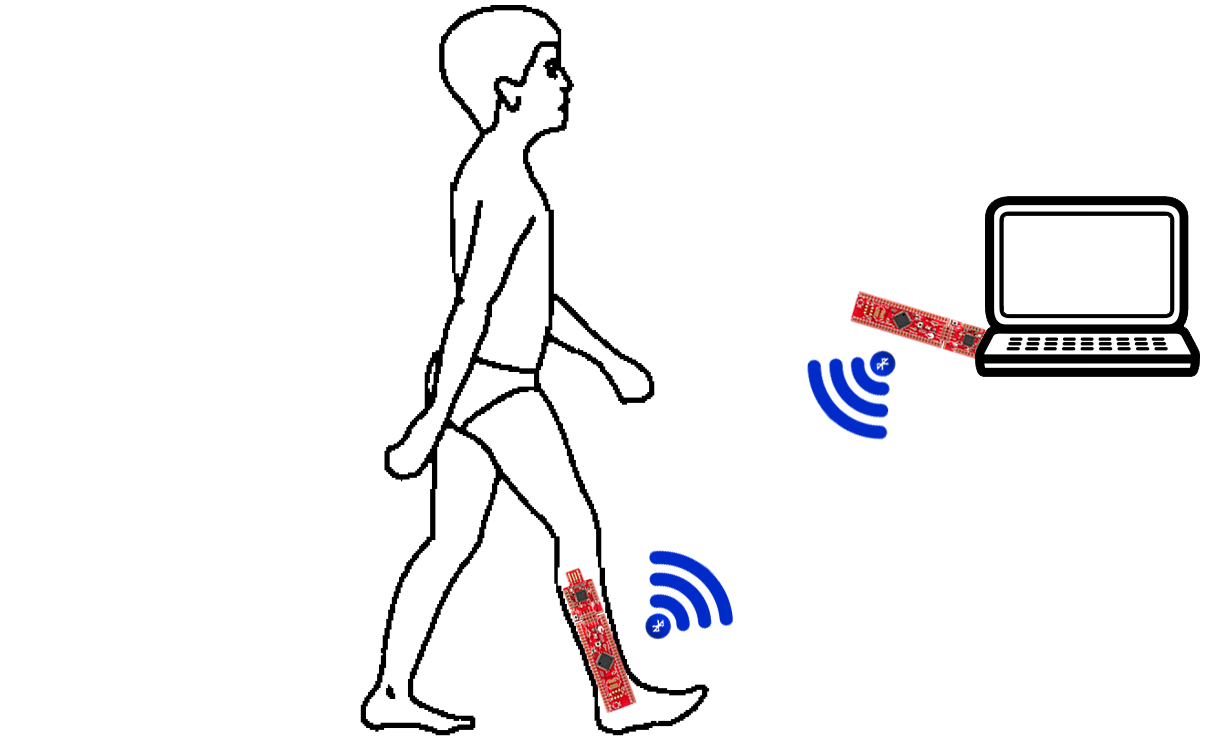
\includegraphics[width=.75\textwidth]{figures/forside2.PNG}
		\end{minipage}
		\hfill
	\end{figure}
	\vspace*{\fill}
	\scshape % Small caps
	{\Large Gruppe 4403\par}
	
	\vspace*{.8\baselineskip} % Whitespace between location/year and editors
	
	Aalborg Universitet,  01/02/2016 - 27/05/2016 \par % Location and year
\end{center} % Center all text
%{\color{white}X \\ X \\ X \\}

%\begin{center}
%	\textit{Gruppemedlemmer:}\\
%	Cecilie Sophie Rosenkrantz Topp, Frederik Skou Nielsen \\
%	Josefine Dam Gade, Line Sofie Hald, Morten Skaarup Larsen
%\end{center}
\begin{center}
	\line(1,0){400}
\end{center}
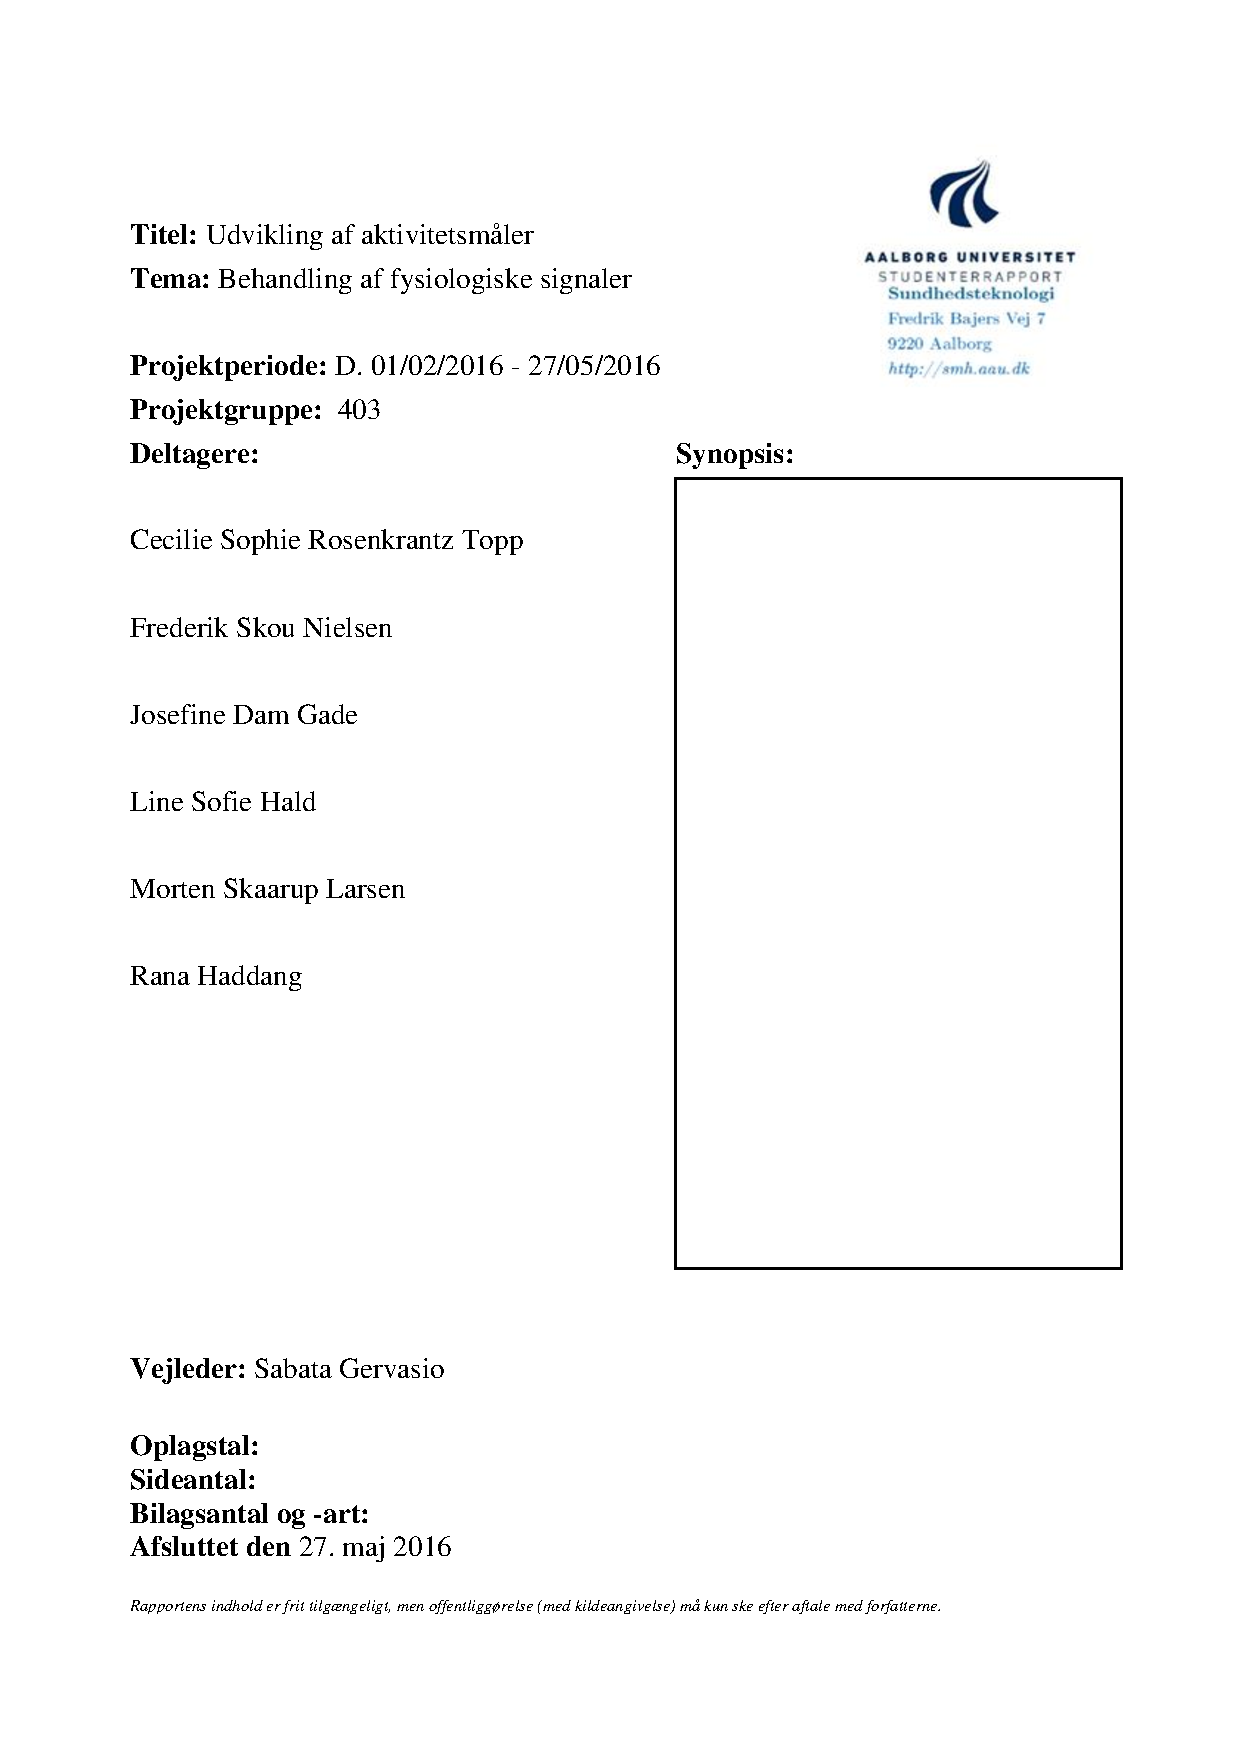
\includepdf[pages={1}]{rapportAfsnit/pFormaliteter/synopsis.pdf} \clearpage 
\chapter*{Forord og læsevejledning}
% !TeX spellcheck = da_DK
\section*{Forord}
Denne rapport er udarbejdet som et 4. semesters projekt på bacheloruddannelsen Sundhedsteknologi, Aalborg Universitet. Projektetperioden forløb fra februar 2016 til maj 2016. \\
Projektet tager udgangspunkt i studieordningen for bacheloruddannelsen i Sundhedsteknologi. Det fremgår, at semesterets fokusområde er 'Behandling af fysiologiske signaler'. Projektgruppen har derfor valgt at 
Dette projekt tager udgangspunkt i projektforslaget 'Udvikling af aktivitetsmåler', hvor formålet blandt andet er design, implementering og test af en prototype, der kan detektere fysisk aktivitet. Protoypen udvikles med henblik på at bestemme det fysisk aktivitetsniveau for børn i aldersgruppe 9-12 år. Prototypen vil derfor involvere en dataopsamling i form af analoge komponenter fra et accelerometer, et gyroskop og en pulssensor. Ydermere vil prototypen indeholde signal- og databehandling som muligøre digital visualisering på et grafisk brugerinterface.

%Projektet henvender sig til studerende på samme niveau eller andre interessere med et kendskab til basal analog og digital databehandling. \\
Der rettes en tak til vejleder Sabata Gervasio for et godt og lærerigt samarbejde under udarbejdelsen af denne rapport. Yderligere rettes der en tak til semesterkoordinater, John Hansen, for råd og vejledning til forståelse af semesterets nye mikrokontroller. 

\section*{Læsevejledning}
Projektet er opbygget af 5 kapitler, litteraturoversigt samt bilag. Før hvert kapitel er der et indledende kursiv afsnit, som har til formål at vejlede læseren i form af det følgende kapitels indhold og sammenhæng i rapportens helhed.\\
Første kapitel består af en indledning og initierende problemstilling. Herefter er problemanalysen, der bearbejder den initierende problemstilling og leder ud i en problemformulering. Det tredje kapitel er problemløsning, hvori blandt andet løsningsstrategi og essentielle teoretiske elementer hertil beskrives. Yderligere indeholder kapitlet krav til protoypen og dets delelementer. Det efterfølgende kapitel består af design, implementering og test af prototpyens delementer samt en test af den samlede prototype. Afslutningsvis er syntesen, indeholdende diskussion, konklusion og perspektivering.

Rapporten benytter Vancouver metoden til kildehenvisning, hvor den første kilde i litteraturoversigten er [1], den næste [2] og så fremdeles. Alle benyttede kilder er at finde i kapitel 5, hvor de er listet i numerisk rækkefølge. I tilfælde, hvor kilden befinder sig inden for punktum, tilhører denne kildehenvisning indholdet i den pågældende sætning sætning. Er kildehenvisningen placeret efter punktummet i sætningen, da tilhører kilden indholdet i det ovenstående afsnit indtil forrige kildehenvisning. \\
Tabeller og figurer er nummereret efter deres respektive afsnit, hvorfor eksempelvis figur 1.1 er den første figur i kapitel 1.

Rapporten benytter forkortelser, hvor ordets fulde længde skrives første gang ordet præsenteres, med tilhørende forkortelse i parantes efter ordet. Efterfølgende vil denne forkortelse benyttes i resten af rapporten, med undtagelse af overskrifter. 
\newpage

%the '*' allows the tableofcontents be excepted from the actual table of contents.
\tableofcontents*

%numbers the pages with Arabic numeral - starts from 1.
\mainmatter
\chapter{Indledning}
% !TeX spellcheck = da_DK
Indledende halløj..

\section{Initierende spørgsmål}
.
% Problemanalyse
\chapter{Problemanalyse}
\section{Fysiologiske konsekvenser}\label{sec:fysio}
Dette afsnit beskriver først, hvilke fysiologiske konsekvenser det kan få for et barn at være inaktiv eller overvægtig. Disse tilstande defineres og beskrives, hvorefter de holdes op mod hinanden. Konsekvenserne ved fysisk aktivitet vil ligeledes blive beskrevet, hvor en forklaring af kognitiv forbedring samt metabolske processer vil indgå.
%I forhistorien, da mennesket var jægere, var der en naturlig favorisering af de mennesker, som kunne lagre fedt bedre end andre, da der kunne gå lang tid imellem måltiderne, hvilket ikke er nødvendigt med den moderne livsstil, hvor teknologi og højere velstand har medført et mere fysisk inaktivt liv samtidig med der er let adgang til føde. Idet evolutionen ikke har tilpasset sig denne moderne livsstil, søger kroppen stadig at lagre fedt, hvorved personer med et lavere aktivitetsniveau end den energi de indtager, langsomt vil ophobe fedtdepoter, hvilket kan resultere i overvægt.\citep{Ahmad2014,Kiens2007}

\subsection{Fysiske konsekvenser ved inaktivitet og overvægt}\label{subsec:inover}
%{\color{red} \textbf{Vi vil sørge for, at dette afsnit fokuserer lidt mere på at man kan både være aktiv men også overvægtig. Desuden vil vi gå lidt mere i dybden med de fysiologiske konsekvenser af at være inaktiv og overvægtig.}}
Danske og internationale studier hævder, at $\sfrac{2}{3}$ drenge og $\sfrac{4}{5}$ piger i aldersgruppen 11-15 år er fysisk inaktive \citep{SundhedsstyrrelsenFaktaark}. Et individ er fysisk inaktiv, hvis vedkommende udfører mindre end 2,5 times fysisk aktivitet om ugen med moderat intensitet, hvilket svarer til 64-74 \% af maxpuls. \citep{Kiens2007}\fxnote{Moderat intensitet svarer til 40-59 \% af den maksimale iltoptagelse, eller 40-59 \% af pulsreserven (maxpuls – hvilepuls), eller 64-74 \% af maxpuls eller 12-13 RPE (rate of percieved excertion, Borgskala) og er yderligere defineret som fysisk aktivitet hvor man bliver lettere forpustet men hvor samtale er mulig} Det er veldokumenteret, at der sker et fald i fysisk aktivitet med alderen samtidig med, at der sker en stigning i vægt\citep{Kaprio2008}. Undersøgelser tyder på, at hvis kroppens cellulære vedligeholdelse styrkes med fysisk aktivitet, så kan aldringsprocessen nedsættes\citep{Knight2012}. Fysisk inaktivitet forstærker altså den generelle aldring og anses som værende mindst lige så farligt som overvægt. De to fænomener forekommer dog ofte samtidig, da inaktivitet kan forsage overvægt, men fysisk inaktivitet har en selvstændig helbredsmæssig betydning ligesom overvægt har. Det er muligt at være overvægtig men samtidig have en aktiv livsstil.\citep{Kaprio2008,Kiens2007,Hjort1997} Undersøgelser viser, at en overvægtig men fit person kan have samme metabolske sundhed, som en normalvægtig. Igennem en aktiv livsstil kan en overvægt nedsætte insulinresistens, højt kolesterol og højt bloktryk, selvom vedkommende forbliver overvægtig. \citep{Lunau2012,Marcelino2012}

Fysisk inaktivitet kan lede til flere af de store folkesygdomme som hjertekarsygdomme, diabetes, osteoporose og psykiske lidelser. Menneskekroppen er ikke skabt til at være inaktiv, og derfor vil kroppen reagere kraftigt på det. For eksempel kan kroppen påbegynde nedbrydelse af knoglerne indefra, så de ikke vejer for meget i forhold til brugen heraf. 60 til 85\% af verdensbefolkningen lever en stillesiddende livsstil, hvilket forstærker forekomsten af disse folkesygdomme.\citep{Kiens2007,Reshma2002,Martini2012} Derudover kan inaktivitet lede til disuse syndromet, som blandt andet indebærer svækket hud integritet, ændret respiratorisk funktion og nedsætning af sanserne\citep{Knight2012,Mosby2009}.

Definitionen for overvægt er globalt sat ud fra et body mass index (BMI), hvilket er forholdet mellem en persons vægt og højde\citep{Academic2016}. Der findes en BMI oversigt for henholdsvis piger og drenge i aldersgruppen 2-20 år, hvorefter grænseområderne for, hvornår en person er undervægtig, normal, overvægtig eller kraftig overvægtig er fast defineret for begge køn. Der er udarbejdet en specifik oversigt for børn i denne aldersgruppe, da et BMI på for eksempel 20 for en femårig ikke er det samme som for en tolvårig. En femårig med dette BMI vil være defineret som kraftig overvægtig, mens en tolvårig vil være inden for den normale zone. Der er ikke signifikant forskel imellem kønnene, men BMI for denne aldersgruppe afhænger meget af alderen. \citep{DiseaseControl2015}\\
Overvægt opstår grundlæggende fordi der indtages mere energi end der forbruges. Nogle mennesker kan lagre fedt bedre end andre, hvorfor overvægt også kan være genetisk betinget.\citep{Nestle2014}\\
Overvægt øger risikoen for højt kolesteroltal, forhøjet blodtryk og diabetes samt følgesygdomme heraf som slagtilfælde og nyresygdomme. Det er dokumenteret, at der er størst risiko for tidlig død jo yngre mennesker opnår overvægt. Det er derfor essentielt at forbedre børns aktivitet og dermed mindske risikoen for overvægt.\citep{Nestle2014} Derudover ses der, at overvægtige børn ofte lider af psykologiske og sociale problemer, hvilket kombineret med overvægten kan have en negativ indvirkning på barnets fremtid i forhold til uddannelse og socioøkonomiske status\citep{Academic2016}.

Inaktivitet kombineret med overvægt øger risikoen for diverse sygdomme, men en normalvægtig inaktiv person er i større risiko for tidlig dødsfald end en overvægt aktiv person. Ifølge et 12-års studie lavet over 334.161 europæiske deltagere så tyder det på, at dobbelt så mange vil dø af inaktivitet end overvægt.\citep{Ekelund2015} En aktiv overvægt person har derudover ikke større chance for at udvikle hjertesygdomme end normalvægtige, så længe de er trænede og dyrker motion\citep{Nichols2014}. Det tyder altså på, at inaktivitet er mere skadeligt end overvægt, hvis de sammenlignes som normalvægtig inaktiv mod overvægtig aktiv.


% !TeX spellcheck = da_DK
\subsubsection{Aktivitet og kognitiv respons}
Fysisk aktivitet har, som det er tilfældet med kroppens fysiske helbred, positive effekter for hjernens kognitive funktioner heriblandt indlæring, hukommelse samt koncentration. %kontrolprocesser, som multitasking, planlægning og koncentration. 
Derudover medvirker længerevarende træningsperioder til en positiv virkning på matematiske færdigheder\fxnote{Matematiske færdigheder} \citep{Bugge2015,Berchtold2010,Schmidt2015}.\\
Måden hvorpå fysisk aktivitet gavner hjernes kognitive funktioner er, at øget fysisk aktivitet resulterer i øget aktivitet i hippocampus, som er lokaliseret i det limbiske system i hjernen. Dette område i hjernen, processerer hukommelse og navigation, hvorved øget fysisk aktivitet forbedrer evnen til indlæring og hukommelse. Ved en længerevarende træningsperiode vil der ske en ændring i hjernens plasticitet, hvorved hjernen adapterer sig til det ændrede aktivitetsniveau\fxnote{Den tilpasser sig til at dyrke mere motion, hvorved området for indlæring og hukommelse vokser - ligesom en muskel man bruger mere}. Blodkarrene i hjernen\fxnote{hippocampus, cortex og cerebellum} udvides, som følge af det øgede aktivitetsniveau, på samme vis som i resten af kroppen\fxnote{reference til fysiologiafsnit}, hvilket medfører at der kan tilføres flere næringsstoffer og mere energi. \citep{Cotman2007}\\
Den fysiske aktivitets effekter på hjernens kognitive funktioner er dog ikke permanente, og aftager langsomt efter aktiviteten er opholdt. Efter fysisk aktivitet i 11-20 minutter, vil de øgede kognitive funktioner for børn vare i op til 50 minutter, mens de for voksne vil vare i 25-45 minutter. \citep{Cotman2007} Ydermere tyder studier på, at fysisk aktivitet kan have en længerevarende positiv effekt på børns kognition \citep{SibleyEtnier2003}.






\begingroup
\raggedright
\bibliographystyle{unsrtnat}
\bibliography{kilder}
\endgroup

\begin{appendices}
\end{appendices}

\end{document}